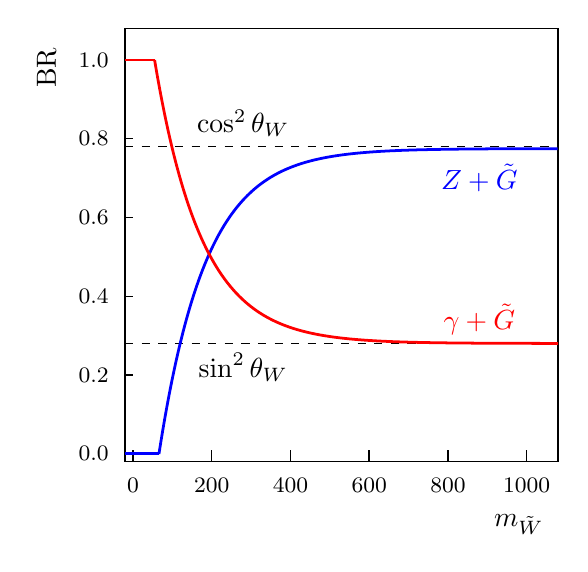
\begin{tikzpicture}

    \tikzstyle{region} = [rounded corners, fill, opacity=0.5, line width=0.1, green]
    \tikzstyle{axis} = [line width=0.6]
    \tikzstyle{tick} = [line width=0.5]
    \tikzstyle{point} = [blue, fill=blue!20]

    \draw[axis] (0,0) -- (5.5,0) node at (5.0,-0.8) {$m_{\tilde{W}}$};
    \draw[axis] (0,0) -- (0,5.5) node[rotate=90] at (-1,5.0) {BR};

    \draw[axis] (5.5,0) -- (5.5,5.5);
    \draw[axis] (0,5.5) -- (5.5,5.5);

    \draw[dashed] (0,1.5) -- (5.5,1.5) node[baseline=left] at (1.5, 1.2) {$\sin^2 \theta_W$};
    \draw[dashed] (0,4.0) -- (5.5,4.0) node[baseline=left] at (1.5, 4.3) {$\cos^2 \theta_W$};


    \draw[tick] (0,5.1) -- (0.1,5.1) node at (-0.4, 5.1) {\footnotesize 1.0};
    \draw[tick] (0,4.1) -- (0.1,4.1) node at (-0.4, 4.1) {\footnotesize 0.8};
    \draw[tick] (0,3.1) -- (0.1,3.1) node at (-0.4, 3.1) {\footnotesize 0.6};
    \draw[tick] (0,2.1) -- (0.1,2.1) node at (-0.4, 2.1) {\footnotesize 0.4};
    \draw[tick] (0,1.1) -- (0.1,1.1) node at (-0.4, 1.1) {\footnotesize 0.2};
    \draw[tick] (0,0.1) -- (0.1,0.1) node at (-0.4, 0.1) {\footnotesize 0.0};

    \draw[tick] (5.1,0) -- (5.1,0.15) node at (5.1,-0.3) {\footnotesize 1000};
    \draw[tick] (4.1,0) -- (4.1,0.15) node at (4.1,-0.3) {\footnotesize 800};
    \draw[tick] (3.1,0) -- (3.1,0.15) node at (3.1,-0.3) {\footnotesize 600};
    \draw[tick] (2.1,0) -- (2.1,0.15) node at (2.1,-0.3) {\footnotesize 400};
    \draw[tick] (1.1,0) -- (1.1,0.15) node at (1.1,-0.3) {\footnotesize 200};
    \draw[tick] (0.1,0) -- (0.1,0.15) node at (0.1,-0.3) {\footnotesize 0};

    \draw[blue, line width=1] (0,0.1) -- (0.43,0.1);
    \draw[blue,line width=1] plot[domain=0.43:5.5, samples=500] ({\x},{1.5*(2.65 - exp(-((\x-1)/0.6)))});

    \draw[red, line width=1] (0,5.1) -- (0.38,5.1);
    \draw[red,line width=1] plot[domain=0.375:5.5, samples=500] ({\x},{1.5+1.5*(exp(-((\x-0.9)/0.6)))});

    \node[blue] at (4.5, 3.6) {$Z+ \tilde{G}$};
    \node[red]  at (4.5, 1.8) {$\gamma + \tilde{G}$};
\end{tikzpicture}
